\documentclass[
	%parspace, % Térköz bekezdések közé / Add vertical space between paragraphs
	%noindent, % Bekezdésének első sora ne legyen behúzva / No indentation of first lines in each paragraph
	%nohyp, % Szavak sorvégi elválasztásának tiltása / No hyphenation of words
	%twoside, % Kétoldalas nyomtatás / Double sided format
	%draft, % Gyorsabb fordítás ábrák rajzolása nélkül / Quicker draft compilation without rendering images
	%final, % Teendők elrejtése / Set final to hide todos
]{elteikthesis}[2020/11/23]

% Dolgozat metaadatai
% Document's metadata
\title{Dolgozat címe} % cím / title
\date{2020} % védés éve / year of defense

% Szerző metaadatai
% Author's metadata
\author{Hallgató Hanga}
\degree{programtervező informatikus BSc}

% Témavezető(k) metaadatai
% Superivsor(s)' metadata
\supervisor{Témavezető Tamás} % belső témavezető neve / internal supervisor's name
\affiliation{egyetemi tanársegéd} % belső témavezető beosztása / internal supervisor's affiliation
%\extsupervisor{Külső Kornél} % külső témavezető neve / external supervisor's name
%\extaffiliation{informatikai igazgató} % külső témavezető beosztása / external supervisor's affiliation

% Egyetem metaadatai
% University's metadata
\university{Eötvös Loránd Tudományegyetem} % egyetem neve / university's name
\faculty{Informatikai Kar} % kar neve / faculty's name
\department{Programozáselmélet és Szoftvertechnológiai\\ Tanszék} % tanszék neve / department's name
\city{Budapest} % város / city
\logo{elte_cimer_szines} % logo

% Irodalomjegyzék hozzáadása
% Add bibliography file
\addbibresource{thesis.bib}

% A dolgozat
% The document
\begin{document}

% Nyelv kiválasztása
% Set document language
\documentlang{magyar}
%\documentlang{english}

% Teendők listája (final dokumentumban nincs)
% List of todos (not in the final document)
%\listoftodos[\todolabel]

% Dokumentum beállítások
% Some document settings
% Lábjegyzet folytonos számozása fejezetek között
% Continuous counting of footnotes among chapters
\counterwithout{footnote}{chapter}

% Tartalomjegyzék oldalszámozásának rejtése
% Hide page numbering of ToC
\newcounter{conpageno}
\let\oldtableofcontents\tableofcontents
\renewcommand{\tableofcontents}{
	\pagenumbering{gobble}
	\oldtableofcontents
	\cleardoublepage
	\setcounter{conpageno}{\value{page}}
	\pagenumbering{arabic}
	\setcounter{page}{\value{conpageno}}
}


% Címlap (kötelező)
% Title page (mandatory)
\maketitle
\topicdeclaration

% Tartalomjegyzék (kötelező)
% Table of contents (mandatory)
\tableofcontents
\cleardoublepage

% Tartalom
% Main content
\chapter{Introduction} % Introduction
\label{ch:intro}

\section{Motivation}

Bugs are more common in programming languages with access to low-level system resources such as C and C++.
A variety of scenarios can result in so-called an undefined or implementation-dependent behavior.
Many examples of such problematic code are hidden in massive language standard specifications and are easily overlooked by inexperienced developers. Not to mention that even well-known bugs (division by zero, use of an uninitialized variable, use after free, etc.) are difficult to detect when they occur not in a single point of the code, but rather in a long chain of events that lead up to it. 

The real issue with undefined behavior (UB) is that a program may behave correctly on some runs but produce runtime errors on others, depending on the compiler, platform, build configurations, and so on. 

In the best-case scenario, UB can cause minor, sometimes even tolerable problems, but it can also be the source of irreparable damage; for example, a crash during an important execution can result in tragedy or severe financial loss.
Patriot Missile Error \cite{patriotmissle}, Knight's 440 Million Error \cite{knight}, Heathrow Terminal 5 Opening \cite{heathrow}, Ariane 5 Flight 501 \cite{ariane}, and many more are well-known examples. Undefined behavior can allow black hat hackers to gain access to confidential information (Hearthbleed \cite{heartbleed}) or run malicious code on the target computer. 

Even if it is difficult, it is still the developer's responsibility to avoid such errors.
Static analyzers, which are automated tools for finding bugs, come to the rescue. 

The goal of this thesis is to extend the open-source static analysis tool so that it can detect three more undefined or implementation-dependent behavior scenarios. 




\section{CERT C/C++ Coding Standard Rules} \label{rules}
The Carnegie Mellon Software Engineering Institute and thousands of researchers and language experts collaborated to create the Secure Coding standard, which describes the root causes of common software vulnerabilities \cite{seicertc} \cite{seicertcpp}.
The following SEI CERT Rules will be addressed in the thesis:
POS34-C \cite{pos34}, ENV31-C \cite{env31}, and ENV34-C \cite{env34}. 

\subsection{POS34-C}
\subsubsection{Do not call putenv() with a pointer to an automatic variable as the argument}

POSIX \cite{posix} function \emph{putenv} is used to change or add environment variables. It accepts only one argument, a pointer to a string of the form "name=value".

\emph{putenv} does not make a copy of the passed string; instead, it adds the pointer to the environment array directly. 
When a pointer to an automatic variable is passed as an argument, a garbage value may end up in the environment because the containing function's stack memory is recycled \cite{putenv}.
This can result in unexpected program behavior or even give the attacker the ability to run arbitrary code. 

\lstset{caption={Pointer to automatic buffer passed to putenv(). Example from CERT rule page.}, label=src:pos34}
\begin{lstlisting}[language={C++}]
int volatile_memory_example(const char *var) {
  char env[1024];
  int retval = snprintf(env, sizeof(env), "TEST=%s", var);
  if (retval < 0 || (size_t)retval >= sizeof(env)) {
    /* Handle error */
  }
  return putenv(env);
}

\end{lstlisting}

\pagebreak

To avoid the issue, programmer has few options: 
\begin{itemize}
	\item Add \lstinline{static} keyword on line 2. 
	\item Use Heap memory allocated pointer as an argument to \lstinline{putenv()}.
	\item Instead of \lstinline{putenv()} favor \lstinline{setenv()} function, which allocates heap memory for environment variables.
\end{itemize}


\subsection{ENV31-C} \label{env31}
\subsubsection{Do not rely on an environment pointer following an operation that may invalidate it}
In ISO C standard \lstinline{main} function takes no arguments, or takes two - \lstinline{int argc} and \lstinline{char *argv[]}; however, in Unix systems, a third argument, \lstinline{char *envp[]}, can be used, which points to the program's environment and has the same value as \lstinline{environ} (global array of environment variables \cite{environ}) \cite{3main}. 

Any change to the environment, such as calling \lstinline{putenv}, \lstinline{setenv}, or their variants, may result in memory being reallocated. \lstinline{environ}  has been updated to reflect this change, but \lstinline{envp} has not, so its use may result in unexpected behavior. 


\lstset{caption={envp pointer used after the modification of environment.}, label=src:cpp1}
\begin{lstlisting}[language={C++}]
int main(int argc, const char *argv[], const char *envp[]) {
  putenv((char *) "VARIABLE=VALUE"); // envp invalidated
  
  if (envp != NULL) {
    for (int i = 0; envp[i] != NULL; ++i) {
      puts(envp[i]);
    }
  }
  return 0;
}

\end{lstlisting}

Developers should keep in mind that changes to the environment will not be reflected in \lstinline{envp} and as an alternative using \emph{environ} (or \emph{\_environ} on Windows standard \cite{wenviron}) is an option.

\subsection{ENV34-C} \label{env34}
\subsubsection{Do not store pointers returned by certain functions}
Some functions copy their results into the internal static buffer and return a pointer to it, but the buffer is overwritten for each subsequent call.
As a result, the previous return value should not be used any longer. 

These functions include \emph{getenv}, \emph{asctime}, \emph{localeconv}, \emph{setlocale} and \emph{strerror}. 

\lstset{caption={Invalidated pointer usage.}, label=src:cpp2}
\begin{lstlisting}[language={C++}]
void invalidated_pointer_usage(){
    char *p, pp;
    p = getenv("VAR1");
    pp = getenv("VAR2"); // p invalidated
    *p; // dereference of invalid pointer
}

\end{lstlisting}

A copy of the first pointer should be created if the programmer wants to use it after the subsequent call.
Another solution would be to use Annex K implementations of these functions, but Annex K is still being discussed, and these functions could ultimately be withdrawn \cite{annexk}. 


\section{Static Analysis}
Static Analysis tools do not run the program, but rather inspect the source or generated binary code at compile time.
It is a broad topic that includes code verification, code transformation, optimization techniques, etc.
However, in this work, we consider static analyzers to be bug-finding tools. 

Static analysis is a difficult, if not impossible, problem.
We can, however, approximate it by employing some heuristics.
This, of course, comes at a cost in the form of False Positives (false reports) and False Negatives (missing some real problems).
Any analyzer tool's goal is to reduce these two as much as possible. 

In this section, we'll go over static analysis techniques and reason why we chose Clang Static Analyzer \cite{clangsa} for this project. 

\subsection{Static Analysis Techniques}

\subsubsection{Textual Pattern Matching}
The concept behind this technique is straightforward. First, the code is converted to canonical form, and then we match different patterns to it. Pattern matching can be used to find relatively simpler errors, for example, if we literally have \emph{" / 0"} in our code. It is very fast and relatively easy to implement. However, such a crude approach will not serve our purpose. 

\subsubsection{AST Matching}
This method attempts to match the abstract syntax tree. AST is an intermediate representation of the code. When compared to textual form, we have much more information available thanks to the compiler, for example, types, templates are resolved, etc. 
The Abstract Syntax Tree of a simple code snippet is shown in figure \ref{fig:clang-ast}. 

\begin{figure}[H]
	\centering
	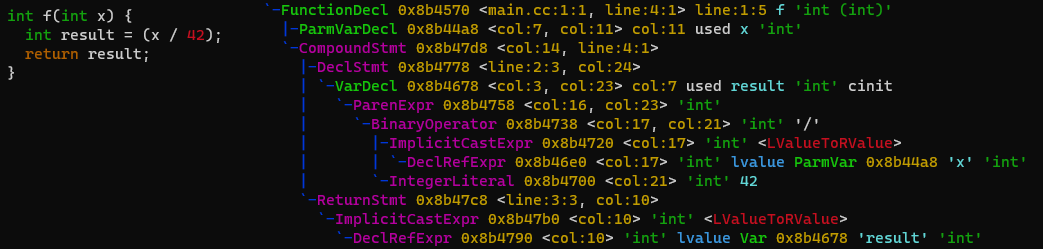
\includegraphics[width=\textwidth]{images/AST_example.png}
	\caption{Clang AST example}
	\label{fig:clang-ast}
\end{figure}


Although AST matching is clearly superior to Textual Pattern Matching, snippet \ref{src:pos34ast} demonstrates that POS34 is a control flow dependent problem that cannot be solved using this technique.
Similar arguments can be made for the other two rules. 



\lstset{caption={POS34 depends on control flow}, label=src:pos34ast}
\begin{lstlisting}[language={C++}]
void foo() {
    char *buffer = "X=Y";
    if (rand() % 2 == 0) {
        buffer = malloc(4);
        strcpy(buffer, "X=Y");
    }
    putenv(buffer); // is buffer on heap or stack?
}
void bar() {
    char *buffer = malloc(4);
    strcpy(buffer, "X=Y");
    if (rand() % 2 == 0) {
        free(buffer);
        buffer = "X=Y";
    }
    putenv(buffer); // is buffer on heap or stack?
}

\end{lstlisting}

\subsubsection{Symbolic Execution}
The Symbolic Execution technique simulates program execution, tries to enumerate every possible execution path, and assigns symbols to represent unknown values. It stores the constraints on symbols (see figure \ref{fig:state}) and eliminates unreachable paths. Such an execution comes at a high cost (exponential in the worst case), but it produces very precise results and allows for the detection of more complex bugs.


\begin{figure}[H]
	\centering
	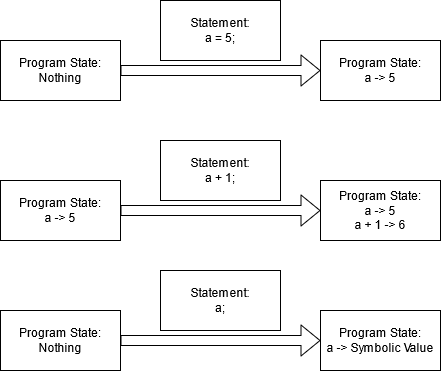
\includegraphics[width=0.6\textwidth]{images/EG.png}
	\caption{How statements affect the program state}
	\label{fig:state}
\end{figure}



\subsection{Clang Static Analyzer}
Clang Static Analyzer is a sophisticated, modern automated tool for detecting flaws in C, C++, and Objective-C codebases.
It is included in the Clang compiler and makes use of all of LLVM's algorithms and data structures. 

The tool is developed and used by technology giants like Ericsson, Apple, Google, Microsoft, Mozilla, and others together with the open-source community and academia.
Clang SA is a path-sensitive analyzer that also performs symbolic execution, has excellent memory modeling \cite{memorym}, and is context-sensitive.
All of this enables Clang Static Analyzer to detect more sophisticated problems, such as bad sequences of events in your program.

Finding the bug is only part of the analyzer's job; equally important is how the tool communicates the report to the developer, especially if it is the result of a long chain of events. 
Clang SA displays the full path, how the problem could have occurred. Figure \ref{fig:div-by-zero} shows analysis result for the Code \ref{src:simple-example}.

Furthermore, the tool is extensible by implementing new modules known as checkers \cite{llvm-dev-meeting}, allowing us to detect new types of bugs.

All of these factors combine to make Clang Static Analyzer an ideal tool for this project. 


\lstset{caption={Invalidated pointer usage.}, label=src:simple-example}
\begin{lstlisting}[language={C++}]
int foo(int x) {
    int y = x;
    if (y == 0) {
        return 1/x;
    }
    return 0;
}

\end{lstlisting}

\begin{figure}[H]
	\centering
	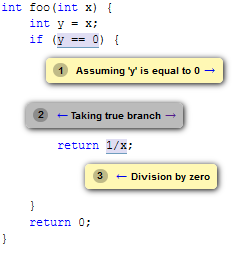
\includegraphics[width=0.6\textwidth]{images/division_by_zero_report.PNG}
	\caption{Static Analyzer warning example}
	\label{fig:div-by-zero}
\end{figure}


\cleardoublepage

\chapter{User Documentation} % User guide
\label{ch:user}


In this chapter, the Clang Static Analyzer will be explained from an end-user perspective. Clang SA is a Clang compiler library that can be found in the LLVM project repository \cite{llvm-project}. 

This work implements two new checkers, \emph{alpha.security.cert.pos.34c} for POS34-C and \emph{alpha.security.cert.env.InvalidPtr} to cover both ENV31-C and ENV34-C. At the time of writing, the first checker is already included in LLVM, while the second is still undergoing official review. 


\section{Install Guide}


\subsection{System Requirements}
Table \ref{tab:sys-req} shows the system requirements and supported compilers for building LLVM. The checkers were developed with Ubuntu 20.04 and tested on Ubuntu 18.04, macOS, and WSL Ubuntu 20.04.


\begin{table}[H]
	\centering
	\begin{tabular}{ | m{0.25\textwidth} | m{0.25\textwidth} | m{0.25\textwidth} |}
		\hline
		\textbf{Operating System} & \textbf{Processor Architecture} & \textbf{Compiler} \\
		\hline \hline
		Linux & x861 & gcc, clang\\
		\hline
		Linux & amd64 & gcc, clang\\
		\hline
		Linux & arm & gcc, clang\\
		\hline
		Linux & Mips & gcc, clang\\
		\hline
		Linux & PowerPC & gcc, clang\\
		\hline
		Solaris & V9 & gcc\\
		\hline
		FreeBSD & x861 & gcc, clang\\
		\hline
		FreeBSD & amd64 & gcc, clang\\
		\hline
		NetBSD & x861 & gcc, clang\\
		\hline
		NetBSD & amd64 & gcc, clang\\
		\hline
		macOS2 & PowerPC & gcc\\
		\hline
		macOS & x86 & gcc, clang\\
		\hline
		Cygwin & x86 & gcc\\
		\hline
		Windows & x86 & Visual Studio\\
		\hline
		Windows64 & x86-64 & Visual Studio\\
		\hline
	\end{tabular}
	\caption{Clang Static Analyzer system requirements}
	\label{tab:sys-req}
\end{table}

\subsection{Building from source}


The commands below will compile LLVM from source. Note that prerequisites are \emph{git}, \emph{CMake} (version 3.4.3 or higher), \emph{gcc} (version 5.1.0 or higher), and \emph{Ninja} build system \cite{ninja}.

\begin{lstlisting}[caption={},label={lst:llvm-build1}]
# on Windows --config core.autocrlf=false flag need to be added to the git clone command.
git clone https://github.com/llvm/llvm-project.git
cd llvm-project

# POS34 checker is already part of LLVM, however for ENV checker user needs to apply git patch
# on top of c79bc5942d0efd4740c7a6d36ad951c59ef3bc0e
# Author: Stefan Pintilie <stefanp@ca.ibm.com>, Date: Tue May 11 05:32:32 2021 -0500
# It could work with the current HEAD of llvm-project, but recent changes might have caused merge conflict.

git checkout c79bc5942d0efd4740c7a6d36ad951c59ef3bc0e
git apply ../invalidPtrChecker.diff

mkdir build
cd build

# Configure build using cmake
cmake \
      -G "Ninja" \
      -DLLVM_ENABLE_PROJECTS="llvm;clang;clang-tools-extra" \
      -DCMAKE_BUILD_TYPE=Release \
      -DBUILD_SHARED_LIBS=ON \
      -DLLVM_TARGETS_TO_BUILD=X86 \
      -DCMAKE_EXPORT_COMPILE_COMMANDS=ON \
      ../llvm/

# -j 4 is number of parallel jobs, user can set it to more.
# It will take a while...
ninja -j 4

# For ease of use the user can add built binaries to the PATH
# export PATH="path/to/llvm-project/build/bin:$PATH"
\end{lstlisting}


\section{Running Analysis} \label{run-analysis}
To demonstrate how to use Clang Static Analyzer, we create main.c file with the following code:

\lstset{caption={}, label=src:trial_run}
\begin{lstlisting}[language={C++}]
#include <stdlib.h>
#include <stdio.h>

int call_putenv(const char *var) {
  char env[1024];
  int retval = snprintf(env , sizeof(env), "TEST=%s", var);
  if (retval < 0) {
    // handle error
  }
  return putenv(env); // putenv function should not be called with auto variables
}

int main(){
  call_putenv("hello clang!");
}
\end{lstlisting}

The simplest way to run Clang SA is to use the clang compiler with the \lstinline{--analyze} option. In order to activate our checkers, we must also include \lstinline{-analyzer-checker=<checker name>} flag. 



\begin{lstlisting}[caption={},label={lst:running-pos34},language={bash}]
clang main.c --analyze \
 -Xclang -analyzer-checker=alpha.security.cert.pos.34c
\end{lstlisting}

If the installation was successful, running the above command gives the following output:

\begin{figure}[H]
	\centering
	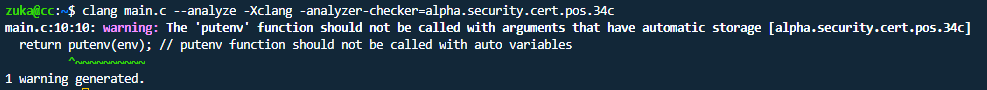
\includegraphics[width=\textwidth]{images/new_pos34.PNG}
	\caption{POS34-C checker output}
	\label{fig:pos34termin}
\end{figure}


Similarly to the POS34-C, the following command can be used to check for ENV31 and ENV34 violations: 
\begin{lstlisting}[caption={},label={lst:running-env}]
clang main.c --analyze \
 -Xclang -analyzer-checker=alpha.security.cert.env.InvalidPtr
\end{lstlisting}

\section{Output options}
More analyzer-specific flags can be added to the invocation commands seen in \ref{run-analysis}.
Users, for example, can choose the best output format for their needs: 
\begin{lstlisting}[caption={},label={lst:output-flag}]
clang main.c --analyze \
 -Xclang -analyzer-checker=alpha.security.cert.env.InvalidPtr \
 -Xclang -analyzer-output=<output type>
\end{lstlisting}

Running the command without the \lstinline{analyzer-output} flag results in default value "none", i.e. it gives warning in standard output as shown in figure \ref{fig:pos34termin}.

\subsection{Text output} \label{text-output}

\lstinline{-analyzer-output=text} still displays the analysis result in the terminal, but it also shows the path diagnostic messages.
Following the actual warning, we can see the steps taken by the symbolic execution that resulted in the bug. 

\begin{figure}[H]
	\centering
	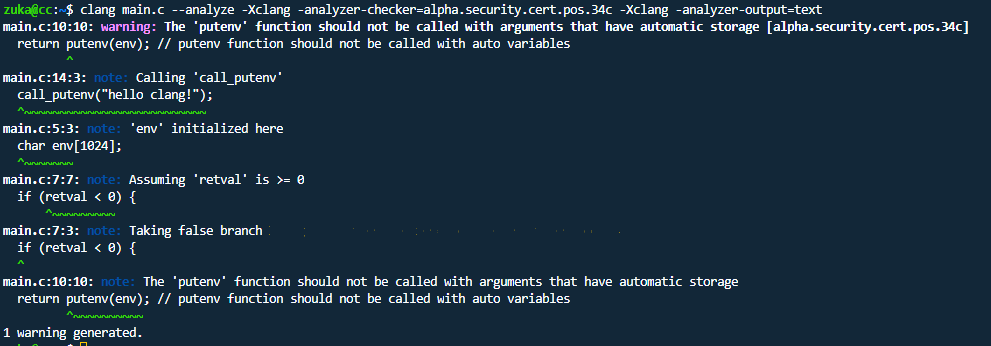
\includegraphics[width=\textwidth]{images/text.PNG}
	\caption{POS34-C with diagnostics}
	\label{fig:pos34termin2}
\end{figure}

\subsection{HTML output} \label{html-output}
The analysis results can also be viewed in HTML format, with a simple graphical interface. 

\begin{lstlisting}[caption={},label={lst:html-output}]
clang main.c --analyze \
 -Xclang -analyzer-checker=alpha.security.cert.env.InvalidPtr
 -Xclang -analyzer-output=html
 -o output/
\end{lstlisting}

If we run the above command will create a new "output" directory (if one does not already exist) where the analysis results will be stored. In our case, it will generate a single (depending on the number of warnings in our source code) HTML file, which will look like this when viewed in a browser: 

\begin{figure}[H]
	\centering
	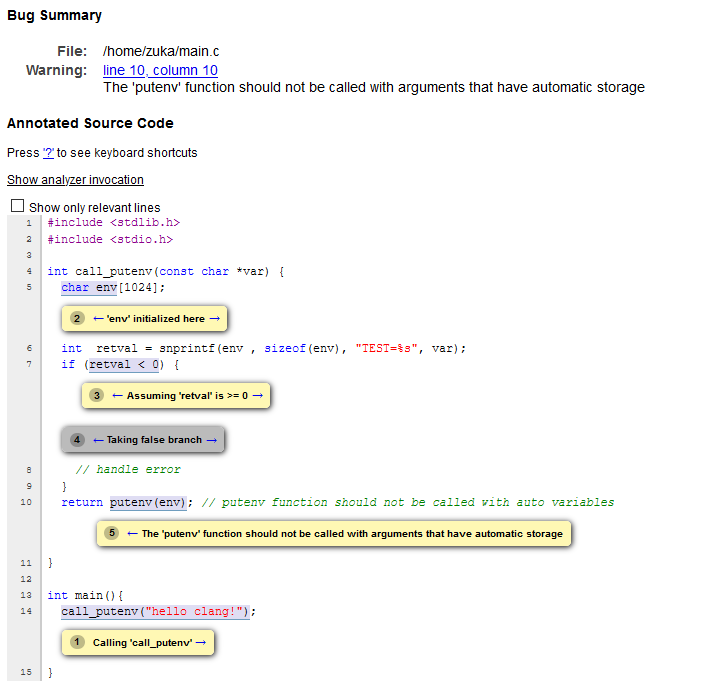
\includegraphics[width=\textwidth]{images/html_out.PNG}
	\caption{HTML output example}
	\label{fig:html-output}
\end{figure}

\subsection{scan-build}
scan-build \cite{scan-build} is a command-line utility that acts as a wrapper around analysis invocation.

The command's general format is as follows: \\
\lstinline{scan-build [scan-build options] <command> [command options]} \\ 
It generates HTML reports and displays warnings in the terminal.

When \lstinline{-o} is not used to specify the output directory, it creates a temp folder with the current timestamp as the name by default. 

Running "scan-view" suggested at the last line of output will start webserver where analysis can be examined.


To browse the list of found bugs, a single index.html file is generated, and by opening a specific report, we see a page similar to figure \ref{fig:html-output}. 


\begin{figure}[H]
	\centering
	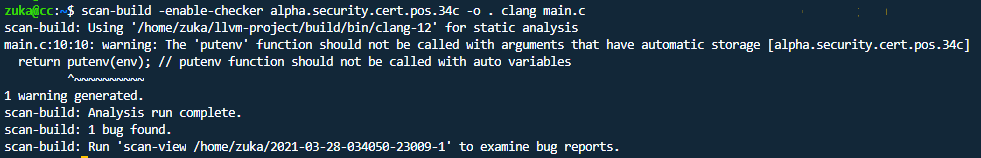
\includegraphics[width=\textwidth]{images/scan-build.PNG}
	\caption{scan-build output}
	\label{fig:scan-build}
\end{figure}


The main benefit of scan-build is that the second part of its invocation can contain any command, allowing users to run static analysis as part of performing a regular build, for example: \\ 
\lstinline{scan-build -enable-checker alpha.security.cert.env.InvalidPtr -o . make -j4} \\
Moreover, \lstinline{--use-analyzer=<path to clang>} flag can also be added, if the user wishes to use the specific clang build version.

\subsection{CodeChecker} \label{codechecker}
Ericsson developed the CodeChecker \cite{cc} tool in collaboration with Eötvös Loránd University to replace the scan-view utility.
In this section, we will show you how to use CodeChecker to analyze an open-source "git" project.

It should be noted that CodeChecker is only available for Linux and Mac OS. 


\subsubsection{Setting up CodeChecker}

To build the CodeChecker from source files, use the following commands: 
\begin{lstlisting}[caption={},label={}, language={bash}]
# prerequisites are npm, virtualenv

git clone https://github.com/Ericsson/CodeChecker.git --depth 1 ~/codechecker
cd ~/codechecker

# create virtual environment and activate it
make venv # or venv_osx for mac
source $PWD/venv/bin/activate

# build codechecker
make package

# optionally user can add it to path for ease of use:
# export PATH="$PWD/build/CodeChecker/bin:$PATH"

cd ..
\end{lstlisting}

\subsubsection{Configuring clang version}
CodeChecker detects and uses the latest available version of Clang that is in the user's path. Since we wish to use the custom-built clang for analysis, we must specify it inside configuration file \lstinline{~/codechecker/build/CodeChecker/config/package_layout.json} Value of "clangsa" should be set to \lstinline{/path/to/llvm-project/build/bin/clang}.


\subsubsection{Running analysis on git}

\lstset{caption={}, label=src:git1}
\begin{lstlisting}[language={bash}]
# install prerequisites for building git
sudo apt-get install gettext
git clone https://github.com/git/git.git
cd git
make configure
./configure --prefix=/usr
CodeChecker log -b "make all -j42" -o compile_commands.json
\end{lstlisting}

The commands above will generate a JSON file containing a compilation database for the git build process. This file is passed to the \lstinline{CodeChecker analyze}, which performs the analysis on each compile command.

\lstset{caption={}, label=src:git2}
\begin{lstlisting}[language={bash}]
CodeChecker analyze \
  /path/to/compile_commands.json \
  --analyzers clangsa \
  --enable alpha.security.cert.env.InvalidPtr \ 
  -o /path/to/output/dir/ \
  -j 42
\end{lstlisting}

This will generate analysis results in .plist files, which can then be converted to HTML with the \lstinline{CodeChecker parse} command. 

\begin{figure}[H]
	\centering
	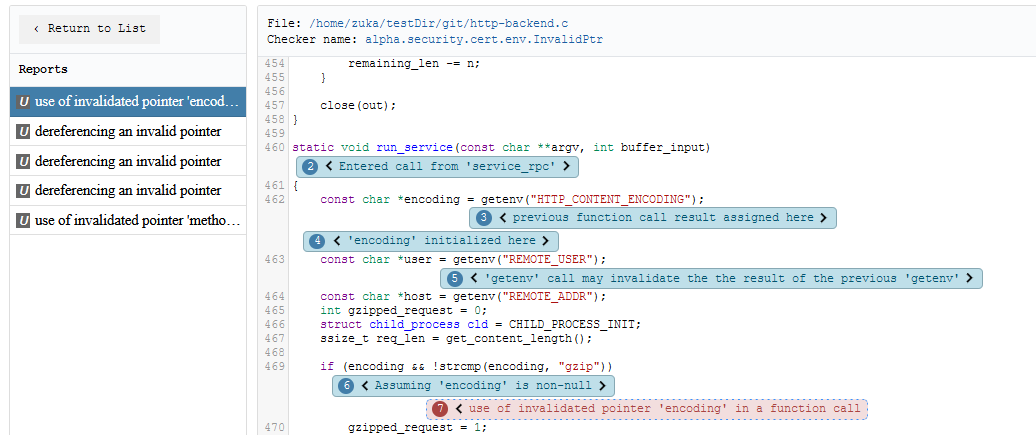
\includegraphics[width=\textwidth]{images/cc_html.PNG}
	\caption{CodeChecker html output}
	\label{fig:cc-html}
\end{figure}

CodeChecker allows users to save analysis results on its server, providing them with a sophisticated graphical interface. 

\lstset{caption={}, label=src:git3}
\begin{lstlisting}[language={bash}]
# start the server on localhost:8555/
CodeChecker server --workspace ./ws --port 8555

# store the analysis results in CC database
CodeChecker store \
  /path/to/plist/files/ \
  --name "project name" \
  --url http://localhost:8555/Default
\end{lstlisting}



\begin{figure}[H]
	\centering
	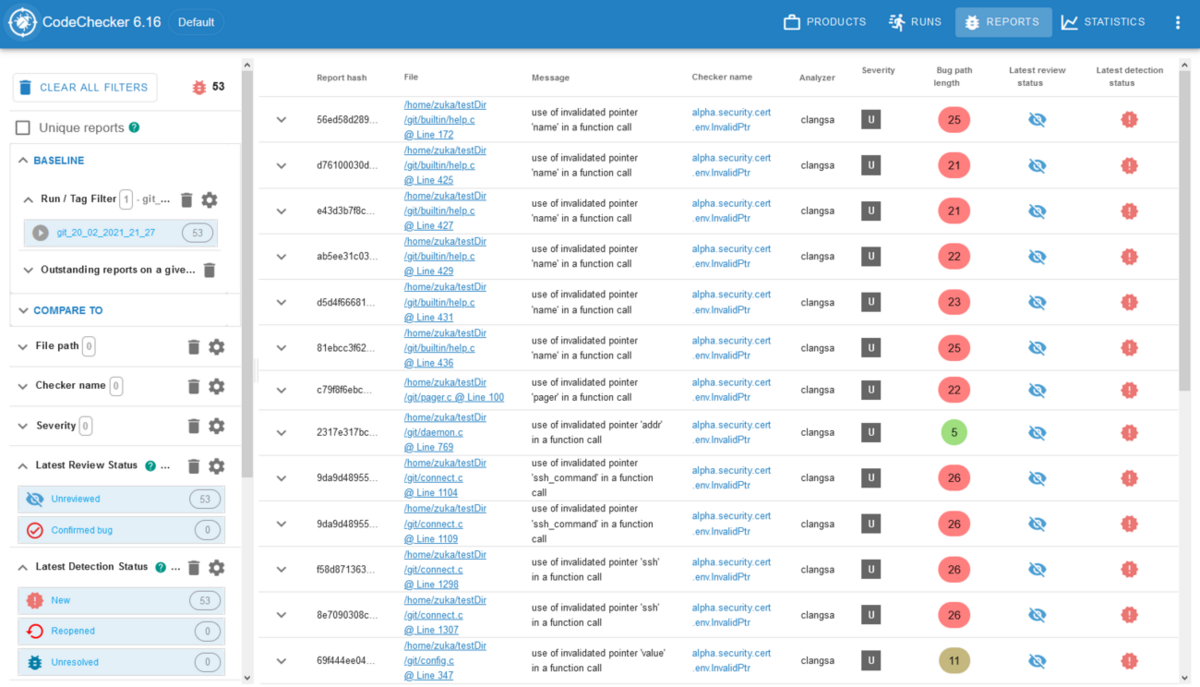
\includegraphics[width=\textwidth]{images/codechecker_reports_new_new.png}
	\caption{CodeChecker graphical user interface, list of reports}
	\label{fig:cc-reports}
\end{figure}

\begin{figure}[H]
	\centering
	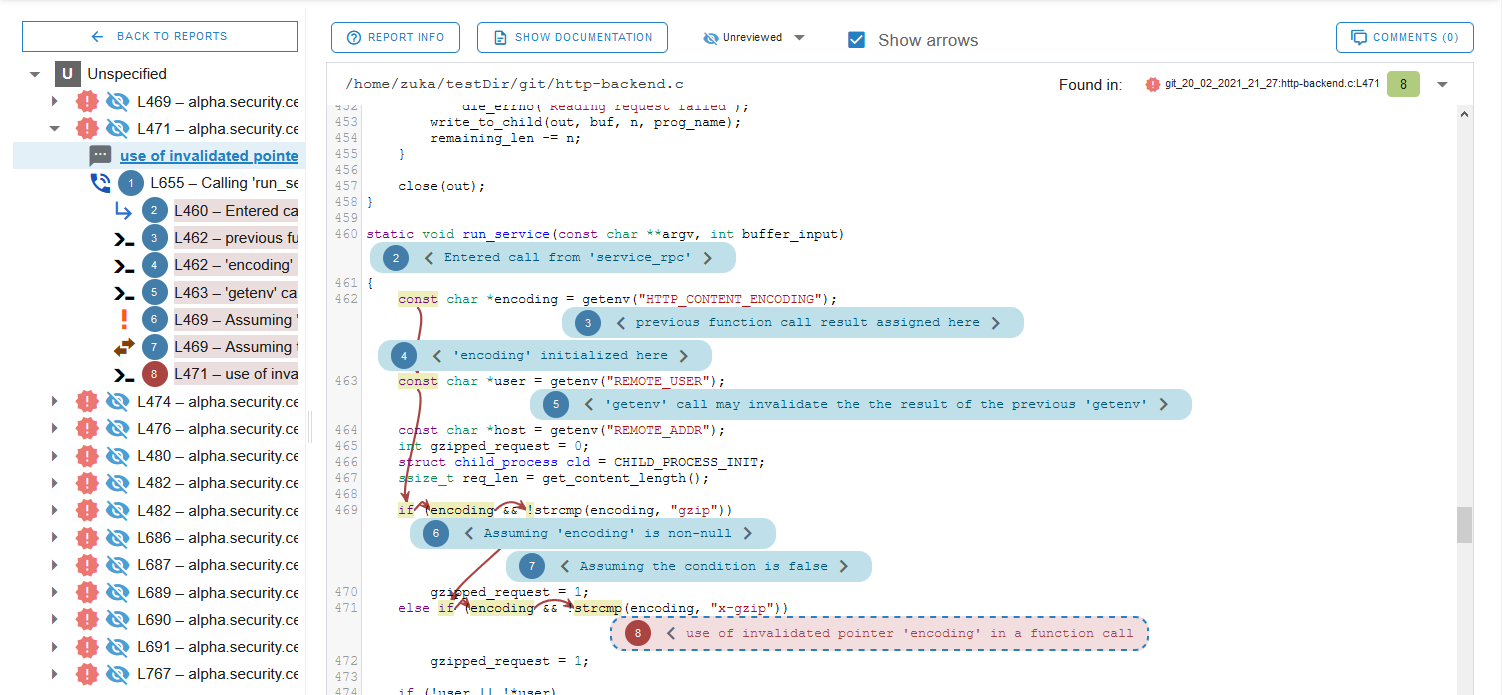
\includegraphics[width=\textwidth]{images/cc_path.PNG}
	\caption{CodeChecker graphical user interface, path diagnostics}
	\label{fig:cc-arrows}
\end{figure}

\cleardoublepage

\chapter{Developer documentation} % Developer guide
\label{ch:impl}

This chapter will cover the basics and the process of developing the Clang Static Analyzer checker. The developer is presumed to have the advanced knowledge of C++, the user experience of Linux, and familiarity with some of the build systems.


\section{Prerequisites}

Before writing the code, the developer must have a few necessary tools.


\begin{itemize}
    \item LLVM repository, available from GitHub \cite{llvm-project}
    \item Git version control system \cite{git}
    \item CMake
    \item Ninja build system. Other build systems can be used as well, however most LLVM developers use ninja 
    \item Development environment of your choice. VS Code, vim, CLion are viable options among others
\end{itemize}


\section{Building Clang} \label{build-clang}

The first step is to checkout LLVM repository from GitHub and create \emph{build}
directory inside. CMake is used to generate build files, it takes few parameters, which are self-explanatory. We use Ninja to start the build process and lastly, it is always a good idea to run all the tests before we start the development process.

\lstset{caption={}, label=build-llvm}
\begin{lstlisting}[language={bash}]
git clone https://github.com/llvm/llvm-project.git

cd llvm-project
mkdir build
cd build

# Configure build using cmake
cmake \
      -G "Ninja" \
      -DLLVM_ENABLE_PROJECTS="llvm;clang;clang-tools-extra" \
      -DCMAKE_BUILD_TYPE=RelWithDebInfo \
      -DBUILD_SHARED_LIBS=ON \
      -DLLVM_TARGETS_TO_BUILD=X86 \
      -DCMAKE_EXPORT_COMPILE_COMMANDS=ON \
      -DLLVM_ENABLE_ASSERTIONS=ON \
      ../llvm/

# -j 4 is number of parallel jobs
# It will take a while...
ninja -j 4

# Run all the tests
ninja check-all -j 4

# For ease of use user can add built binaries to the PATH
# export PATH="path/to/llvm-project/build/bin:$PATH"
\end{lstlisting}

The above steps will build clang along with some useful tools for development and testing. Later on, it is enough to rebuild just clang using \lstinline{ninja clang -j 4} while running only clang analysis specific tests is possible with \lstinline{ninja check-clang-analysis}


\section{Clang Static Analyzer Basics}
 
\subsection{Exploded Graph}
Static Analysis starts with reading plain source code, which is later transformed to Abstract Syntax Tree by Clang. Clang-Tidy, another LLVM native static analyzer tool, is using AST to find bugs in a source code, however, Clang SA takes a different approach and dives into Control Flaw Graph. Clang's CFG is a data structure that consists of AST statements, which are ordered as they are actually executed (figure \ref{fig:ast-and-cfg}). CFG is used by Clang to produce some compiler warnings, but Static Analyzer goes one step further and produces a new data structure called Exploded Graph. It essentially represents the result of the analysis, hence Clang Static Analyzer can be seen as a converter from AST to the Exploded Graph. Finding a bug in the source code is reduced to solving the graph reachability problem.

Exploded Graph consists of paths through CFG. Nodes are pairs of Program Point (the point between two statements, i.e. we finished the first but haven't started evaluating the second) and Program State (the big picture: how already evaluated statements affected the analysis).


\begin{figure}[H]
	\centering
	\subfigure[AST and CFG of x + y + z]{
		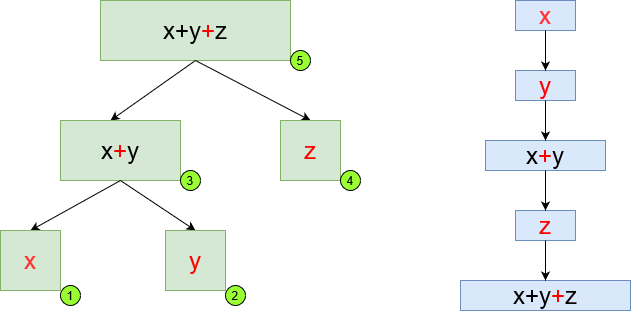
\includegraphics[width=\textwidth]{images/CFG_AST.png}}
	\hspace{30pt}
	\subfigure[AST and CFG of x ? y : z]{
		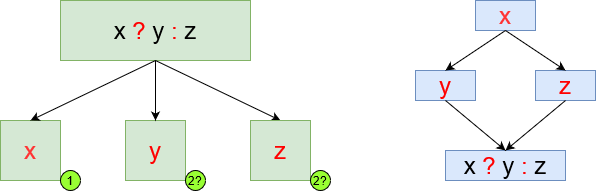
\includegraphics[width=\textwidth]{images/CFG_AST2.png}}
	\caption{Comparison of AST and CFG}
	\label{fig:ast-and-cfg}
\end{figure}

\subsection{Checkers}
Checkers are independent analyzer modules. They inherit from a template class \lstinline{Checker}; the template parameters are types of events to which checker is subscribed. For example, if a checker is interested in an event that occurs after a function call is processed, it can inherit from \lstinline{Checker<check::PostCall>} and implement \lstinline{checkPostCall} to inspect the event, issue a warning if necessary, or provide additional information to the analysis (checkers are active participants in the graph building process). The Checker Developer's Guide \cite{noqa} contains a list of all such callbacks as well as examples of their use. 

\subsection{Custom Program States} \label{checker-states}
During the analysis there is no guarantee about the order in which the program will be explored, or even that all possible paths will be explored; As a result, when checkers need to keep track of information specific to their work, it can not be stored within a single checker class. Instead, they add the data to \lstinline{ProgramState}. There are few macros designed for this purpose:

\begin{itemize}
    \item \lstinline{REGISTER_TRAIT_WITH_PROGRAMSTATE} -- Used when the state information is a single value.
    \item \lstinline{REGISTER_LIST_WITH_PROGRAMSTATE} -- Used when the state information is a list of values.
    \item \lstinline{REGISTER_SET_WITH_PROGRAMSTATE} -- Used when the state information is a set of values.
    \item \lstinline{REGISTER_MAP_WITH_PROGRAMSTATE} -- Used when the state information is a map from a key to a value.
\end{itemize}

All the above data structures come with convenient getter and setter functions. However, since \lstinline{ProgramState} is immutable, whenever we modify the data inside it, a copy of the state with the change applied is created. By calling the \lstinline{CheckerContext::addTransition} function, the updated state must be returned to the analyzer core. 

\section{Implementation}
This section describes the implementation of alpha.security.cert.pos.34c and alpha.security.cert.env.InvalidPtr checkers. 

\subsection{alpha.security.cert.pos.34c} \label{putenv}

The idea behind this checker is straightforward, and as one of the LLVM reviewers put it, "the source code reads so easily, we might as well put it as the official CERT rule description".
We subscribe for function call events, determine if it is \lstinline{putenv}, and inspect its argument, see figure \ref{fig:putenv-diag}.


\begin{figure}[H]
	\centering
	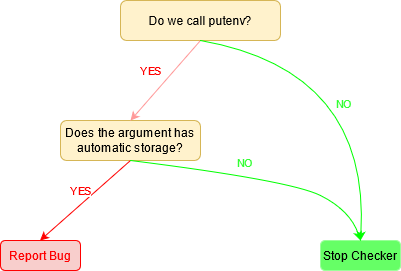
\includegraphics[]{images/putenv_diagram.png}
	\caption{PutenvWithAuto checker logic}
	\label{fig:putenv-diag}
\end{figure}

We use \lstinline{void checkPostCall(const CallEvent &Call, CheckerContext &C)} callback, which passes control to the checker after any function call.

\lstinline{CallEvent::isCalled()} function takes \lstinline{CallDescription} type as an argument and determines whether the called function matches one in the argument. To accomplish this, we first represent \lstinline{putenv} as \lstinline{CallDescription}.

\lstset{caption={}}
\begin{lstlisting}[language={C++}]
class PutenvWithAutoChecker : public Checker<check::PostCall> {
private:
    // ...
    const CallDescription Putenv{"putenv", 1};
public:
  void checkPostCall(const CallEvent &Call, CheckerContext &C) const;
};
void PutenvWithAutoChecker::checkPostCall(const CallEvent &Call,
                                          CheckerContext &C) const {
    if (!Call.isCalled(Putenv))
        return;                                      
    // ...
}
\end{lstlisting}

If the called function matches \lstinline{putenv}, we proceed to the argument, which is represented as \lstinline{SVal}.
We find the \emph{Memory Space Region} of this \lstinline{SVal} and compare it to the \lstinline{StackSpaceRegion}, the base class of everything stored on a stack.

\lstset{caption={}}
\begin{lstlisting}[language={C++}]
void PutenvWithAutoChecker::checkPostCall(const CallEvent &Call,
                                          CheckerContext &C) const {
    // ...
    SVal ArgV = Call.getArgSVal(0);
    const MemSpaceRegion *MSR = 
                    ArgV.getAsRegion()->getMemorySpace();
    if (!isa<StackSpaceRegion>(MSR))
        return;
    // ...
}
\end{lstlisting}

If we passed the both return statements in the preceding code snippets, we have violated POS34-C, as described in section \ref{rules}, and we must report the bug.

This is accomplished by creating \lstinline{PathSensitiveBugReport}, which takes three parameters:

\begin{enumerate}
    \item The type of a bug, instance of \lstinline{BugReport} class.
    \item Short descriptive error message.
    \item \lstinline{ExplodedNode}, the context in which the problem happened. This includes the location of the bug and the current state.
\end{enumerate}

After \lstinline{BugReport} is created, it must be passed to the analyzer core by \lstinline{CheckerContext::emitReport} function.

\lstset{caption={}}
\begin{lstlisting}[language={C++}]
class PutenvWithAutoChecker : public Checker<check::PostCall> {
private:
    BugType BT{this, "'putenv' function should not be called with auto variables", categories::SecurityError};
    // ...
};

void PutenvWithAutoChecker::checkPostCall(const CallEvent &Call,
                                          CheckerContext &C) const {
    // ...
    StringRef ErrorMsg = "The 'putenv' function should not be called with arguments that have automatic storage";
    ExplodedNode *N = C.generateErrorNode();
    auto Report = std::make_unique<PathSensitiveBugReport>(BT, ErrorMsg, N);
    C.emitReport(std::move(Report));
}
\end{lstlisting}

As a next step, we register the new checker by including two boilerplate functions to the source code: 
\lstset{caption={}}
\begin{lstlisting}[language={C++}]
void ento::registerPutenvWithAuto(CheckerManager &Mgr) {
  Mgr.registerChecker<PutenvWithAutoChecker>();
}

bool ento::shouldRegisterPutenvWithAuto(const LangOptions &) { 
    return true; 
}
\end{lstlisting}

By adding it to \lstinline{lib/StaticAnalyzer/Checkers/CMakeLists.txt}, the source code file is made visible to CMake.


Finally, inside \lstinline{include/clang/StaticAnalyzer/Checkers/Checkers.td} we select a package for the checker. The "CERT" package was created as a child of "SecurityAlpha," and it has two children, "POS" and "ENV" for our two checkers, respectively, as shown in the figure \ref{fig:packages}. One can verify that new checker was added by checking available checkers: \lstinline{clang -cc1 -analyzer-checker-help}.


\begin{figure}[H]
	\centering
	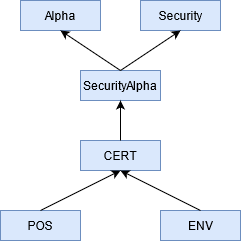
\includegraphics[]{images/packages.png}
	\caption{Checker packages tree}
	\label{fig:packages}
\end{figure}


\subsection{alpha.security.cert.env.InvalidPtr} \label{invalidptr}
A close examination of rules ENV31-C in section \ref{env31} and ENV34-C in section \ref{env34} reveals that they are very similar.
In both cases, some sequence of events invalidates pointers, and subsequent dereference of these invalid pointers results in unintended behavior. Furthermore, there are several scenarios in which a pointer escapes analysis, such as when it is passed to a function that cannot be analyzed. To further reduce false negatives we will add one more heuristic and issue a warning when an invalidated pointer is used as an argument to a function that is not conservatively evaluated. 

Assuming we have a collection of invalidated pointers, we can use the same logic to check for usage and issue a warning in both cases, as shown in figure \ref{fig:invalidptr}. This inspires us to create a single checker that handles both rules. 

\begin{figure}[H]
	\centering
	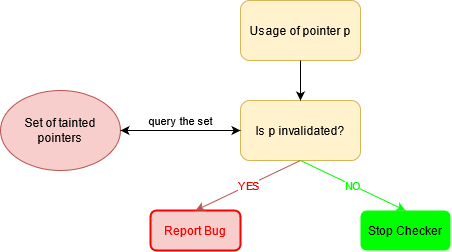
\includegraphics[]{images/invalid_ptr.png}
	\caption{High level logic of InvalidPtr checker}
	\label{fig:invalidptr}
\end{figure}


\subsubsection{Invalidating pointer -- ENV31-C} \label{invalidate-env31}
The first step is to get the \lstinline{envp} argument of \lstinline{main}, if it exists. For this we use \lstinline{checkBeginFunction}, which is called when the core begins to analyze a function. We check if function is \lstinline{main} and store third argument inside the state.

\lstset{caption={}}
\begin{lstlisting}[language={C++}]
// Stores the region of the environment pointer of 'main' (if present).
// Note: This pointer has type 'const MemRegion *'
REGISTER_TRAIT_WITH_PROGRAMSTATE(EnvPtrRegion, const void *)

void InvalidPtrChecker::checkBeginFunction(CheckerContext &C) const {
  if (!C.inTopFrame())
    return;

  const auto *FD = dyn_cast<FunctionDecl>(C.getLocationContext()->getDecl());
  if (!FD || FD->param_size() != 3 || !FD->isMain())
    return;

  ProgramStateRef State = C.getState();
  const MemRegion *EnvpReg =
      State->getRegion(FD->parameters()[2], C.getLocationContext());

  // Save the memory region pointed by the environment pointer
  State = State->set<EnvPtrRegion>(
      reinterpret_cast<void *>(const_cast<MemRegion *>(EnvpReg)));
  C.addTransition(State);
}
\end{lstlisting}

The next step is to move the \lstinline{envp} pointer to an invalidated set, if an environment modifying function is called,
Such functions are stored in \lstinline{CallDescriptionMap}, which is a map from \lstinline{CallDescription} to their handler functions.
Similarly to POS34-C, we use \lstinline{checkPostCall} to listen for function calls and, if it is found in our map, we call the handler. 


\lstset{caption={}}
\begin{lstlisting}[language={C++}]
  void EnvpInvalidatingCall(const CallEvent &Call, CheckerContext &C) const;
  using HandlerFn = void (InvalidPtrChecker::*)(const CallEvent &Call, CheckerContext &C) const;
  const CallDescriptionMap<HandlerFn> EnvpInvalidatingFunctions = {
      {{"setenv", 3}, &InvalidPtrChecker::EnvpInvalidatingCall},
      {{"unsetenv", 1}, &InvalidPtrChecker::EnvpInvalidatingCall},
      {{"putenv", 1}, &InvalidPtrChecker::EnvpInvalidatingCall},
      {{"_putenv_s", 2}, &InvalidPtrChecker::EnvpInvalidatingCall},
      {{"_wputenv_s", 2}, &InvalidPtrChecker::EnvpInvalidatingCall},
  };
  
  void InvalidPtrChecker::checkPostCall(const CallEvent &Call, CheckerContext &C) const {
    // Check if function invalidates 'envp' argument of 'main'
    if (const auto *Handler = EnvpInvalidatingFunctions.lookup(Call))
      (this->**Handler)(Call, C);
    // ...
  }
  
  void InvalidPtrChecker::EnvpInvalidatingCall(const CallEvent &Call, CheckerContext &C) const {
    // check if EnvPtrRegion exists
    // add it to the set of invalidated pointers
  }
\end{lstlisting}

\subsubsection{Invalidating pointer -- ENV34-C}

Aside from the five functions mentioned in the rule, many non-reentrant C library functions suffer from a similar problem.
This part of the checker was designed with genericness in mind, so that simply adding a new entry to the \lstinline{CallDescriptionMap} is sufficient to extend the checker. 


\lstset{caption={}}
\begin{lstlisting}[language={C++}]
  const CallDescriptionMap<EvalFn> PreviousCallInvalidatingFunctions = {
      {{"getenv", 1}, &InvalidPtrChecker::evalGetenv},
      {{"setlocale", 2}, &InvalidPtrChecker::evalSetlocale},
      {{"strerror", 1}, &InvalidPtrChecker::evalStrerror},
      {{"localeconv", 0}, &InvalidPtrChecker::evalLocaleconv},
      {{"asctime", 1}, &InvalidPtrChecker::evalAsctime},
  };
\end{lstlisting}

We create a custom map in which the keys are function names and the values are the results of the most recent call to this function: \\
\lstinline{REGISTER_MAP_WITH_PROGRAMSTATE(PreviousCallResultMap, const char *, const MemRegion *)} \\

On each call to the problematic function, we move the previous value (if it exists) from \lstinline{PreviousCallResultMap} to the invalidated set and update the map with the new memory region. 

\subsubsection{Reporting a bug}

Every time a specific memory location is accessed, the \lstinline{checkLocation} callback is triggered. Inside it we check if accessed memory is invalidated and report dereference of an invalidated pointer if it is. \\



\lstset{caption={}}
\begin{lstlisting}[language={C++}]
  void InvalidPtrChecker::checkLocation(SVal Loc, bool isLoad, const Stmt *S,
                                      CheckerContext &C) const {
  ProgramStateRef State = C.getState();

  // Ignore memory operations involving 'non-invalidated' locations.
  const MemRegion *InvalidatedSymbolicBase =
      findInvalidatedSymbolicBase(State, Loc.getAsRegion());
  if (!InvalidatedSymbolicBase)
    return;

  ExplodedNode *ErrorNode = C.generateNonFatalErrorNode();
  if (!ErrorNode)
    return;

  auto Report = std::make_unique<PathSensitiveBugReport>(
      BT, "dereferencing an invalid pointer", ErrorNode);
  C.emitReport(std::move(Report));
}
\end{lstlisting}

We also issue a warning whenever an invalidated pointer is passed as an argument to a non-conservatively analyzed function, as mentioned in \ref{invalidptr}.
We do this within \lstinline{checkPostCall} by traversing the array of arguments of a function and querying \lstinline{InvalidatedPointerSet} for each of them. 


% TODO
% \subsubsection{Path Diagnostics}
% To make the reports user friendly, custom visitor is implemented, which traverses the graph in search of invalidating function call and adds notes at the point of invalidation. 

% Next step is to make the report user friendly by adding notes, just like in figure \ref{fig:pos34termin2}. For POS34 we relied on built in \lstinline{bugreporter::trackExpressionValue()} for generating such a notes for the problematic \lstinline{putenv} argument, however for InvalidPtr we have to do it manually by creating   



\section{Testing}

Clang Static Analyzer checker testing consists of two parts: lit testing (see \ref{lit}) and running analysis on large code bases to find real world bug examples and, more importantly, to see if the analyzer breaks (see \ref{codebases}). 

\subsection{Lit} \label{lit}

The idea behind lit testing is simple: we create test files with faulty source code and specify which lines should generate a warning or a note.
Clang's \lstinline{-verify} flag performs this type of verification.
Consider the following example: 

\lstset{caption={}}
\begin{lstlisting}[language={C++}]
void getenv_test() {
  char *p1, *p2, *p3;

  p1 = getenv("VAR1");
  *p1; // no-warning

  p1 = getenv("VAR2"); // expected-note{{previous function call was here}}
  p3 = getenv("VAR3"); // expected-note{{'getenv' call may invalidate the the result of the previous 'getenv'}}

  p2 = getenv("VAR4");

  *p1; // expected-warning{{dereferencing an invalid pointer}}
}
\end{lstlisting}

Compliant code must also be tested; typically, a "no-warning" comment is written on lines that may be problematic; however, this is just a convention among analyzer developers and has no actual meaning behind it. 

\lstinline{expected-note} and \lstinline{expected-warning} are sometimes referred as verify comments. It is also possible to pass them some optional arguments, such as the distance between the comment and the actual warning, or the number of times the analyzer should throw an error.
For a better illustration, consider the following slightly modified version of the preceding example: 

\begin{lstlisting}[language={C++}]
void getenv_test1() {
  char *p1, *p2, *p3;

  p1 = getenv("VAR1");
  *p1; // no-warning

  p1 = getenv("VAR2");
  // expected-note@-1{{previous function call was here}}
  p3 = getenv("VAR3");
  // expected-note@-1{{'getenv' call may invalidate the the result of the previous 'getenv'}}

  p2 = getenv("VAR4");
  
  // expected-note@+1{{dereferencing an invalid pointer}}
  *p;
  // expected-warning@-1{{dereferencing an invalid pointer}}
}

\end{lstlisting}

\subsubsection{LLVM Integrated Tester}
llvm-lit is a lightweight tool for LLVM black box testing.

Each lit test file should begin with the following comment:
\lstinline{// RUN: <command>}, where command is argument for llvm-lit to run in terminal. 

\begin{lstlisting}[language={C++}]
// RUN: %clang_analyze_cc1 \
// RUN:  -analyzer-checker=alpha.security.cert.env.InvalidPtr\
// RUN:  -analyzer-output=text -verify %s
\end{lstlisting}


\lstinline{clang_analyze_cc1} is a macro that replaces analyzer invocation.
On the third line, the output type text is specified to check for issued notes as well as warnings (see \ref{text-output}), and the \lstinline{-verify} flag is enabled. 


ENV31-C (section \ref{env31}) states that pointers can be invalidated by operations that modify the environment, but there are a few ways to do so.
To avoid code duplication and having a similar test for each env modifying function, we use the macro \lstinline{ENV_INVALIDATING_CALL}, which takes different values on different lit invocations. This is the test file for this rule: 

\begin{lstlisting}[language={C++}]
// RUN: %clang_analyze_cc1 -analyzer-output=text %s\
// RUN:  -analyzer-checker=core,alpha.security.cert.env.InvalidPtr\
// RUN:  -verify=putenv,common\
// RUN:  -DENV_INVALIDATING_CALL="putenv(\"X=Y\")"
//
// RUN: %clang_analyze_cc1 -analyzer-output=text %s \
// RUN: -analyzer-checker=core,alpha.security.cert.env.InvalidPtr\
// RUN: -verify=putenvs,common\
// RUN: -DENV_INVALIDATING_CALL="_putenv_s(\"X\", \"Y\")"
//
// RUN: %clang_analyze_cc1 -analyzer-output=text %s\
// RUN: -analyzer-checker=core,alpha.security.cert.env.InvalidPtr\
// RUN: -verify=wputenvs,common\
// RUN: -DENV_INVALIDATING_CALL="_wputenv_s(\"X\", \"Y\")"
//
// RUN: %clang_analyze_cc1 -analyzer-output=text %s\
// RUN: -analyzer-checker=core,alpha.security.cert.env.InvalidPtr\
// RUN: -verify=setenv,common\
// RUN: -DENV_INVALIDATING_CALL="setenv(\"X\", \"Y\", 0)"
//
// RUN: %clang_analyze_cc1 -analyzer-output=text %s\
// RUN: -analyzer-checker=core,alpha.security.cert.env.InvalidPtr\
// RUN: -verify=unsetenv,common\
// RUN: -DENV_INVALIDATING_CALL="unsetenv(\"X\")"

// ...
// Function and type definitions
// ...

void call_env_invalidating_fn(char **e) {
  ENV_INVALIDATING_CALL;
  // putenv-note@-1 5 {{'putenv' call may invalidate the environment parameter of 'main'}}
  // putenvs-note@-2 5 {{'_putenv_s' call may invalidate the environment parameter of 'main'}}
  // wputenvs-note@-3 5 {{'_wputenv_s' call may invalidate the environment parameter of 'main'}}
  // setenv-note@-4 5 {{'setenv' call may invalidate the environment parameter of 'main'}}
  // unsetenv-note@-5 5 {{'unsetenv' call may invalidate the environment parameter of 'main'}}

  *e;
  // common-warning@-1 {{dereferencing an invalid pointer}}
  // common-note@-2 {{dereferencing an invalid pointer}}
}

int main(int argc, char *argv[], char *envp[]) {
  char **e = envp;
  *e;    // no-warning
  e[0];  // no-warning
  *envp; // no-warning
  call_env_invalidating_fn(e);
  // common-note@-1 5 {{Calling 'call_env_invalidating_fn'}}
  // common-note@-2 4 {{Returning from 'call_env_invalidating_fn'}}

  *e;
  // common-warning@-1 {{dereferencing an invalid pointer}}
  // common-note@-2 {{dereferencing an invalid pointer}}

  *envp;
  // common-warning@-1 2 {{dereferencing an invalid pointer}}
  // common-note@-2 2 {{dereferencing an invalid pointer}}

  fn_without_body(e);
  // common-warning@-1 {{use of invalidated pointer 'e' in a function call}}
  // common-note@-2 {{use of invalidated pointer 'e' in a function call}}

  fn_with_body(e); // no-warning
}
\end{lstlisting}


It is worth noting that the \lstinline{verify} flag accepts optional arguments and asserts only those comments on each run. 

Following command can be used to run all POS34 and InvalidPtr tests:  \\ 
\lstinline{llvm-lit path/to/llvm-project/clang/test/Analysis/cert  -a}


\begin{table}[H]
	\centering
	\begin{tabular}{ | m{0.15\textwidth} | m{0.40\textwidth} | m{0.40\textwidth} |}
		\hline
		\textbf{Test case} & \textbf{Source file, line} & \textbf{Description} \\
		\hline \hline
		putenv & pos34-c-fp-suppression.cpp, 13 & no warning on extern variable\\
		\hline
		putenv & pos34-c-fp-suppression.cpp, 18 & no warning on non-auto variable\\
		\hline
		putenv & pos34-c-fp-suppression.cpp, 27 & no warning on non-auto variable\\
		\hline
		putenv & pos34-c-fp-suppression.cpp, 38 & false positive, marked as todo\\
		\hline
		putenv & pos34-c.cpp, 16 & warn on volatile variable, example from CERT\\
		\hline
		putenv & pos34-c.cpp, 31 & no warning on static variable, example from CERT\\
		\hline
		putenv & pos34-c.cpp, 42 & no warning on heap variable, example from CERT\\
		\hline
	\end{tabular}
	\caption{Summary of automated tests for POS34-C}
	\label{tab:tests1}
\end{table}


\begin{table}[H]
	\centering
	\begin{tabular}{ | m{0.30\textwidth} | m{0.20\textwidth} | m{0.50\textwidth} |}
		\hline
		\textbf{Test case} & \textbf{Source file, line} & \textbf{Description} \\
		\hline \hline
		putenv, putenv\_s, wputenv\_s, setenv, unsetenv & env31-c.c, 46 & warn dereference of invalidated pointer\\
		\hline
		putenv, putenv\_s, wputenv\_s, setenv, unsetenv & env31-c.c, 60 & warn dereference of invalidated pointer after returning from function call\\
		\hline
		putenv, putenv\_s, wputenv\_s, setenv, unsetenv & env31-c.c, 64 & warn dereference of alias of invalidated pointer\\
		\hline
		putenv, putenv\_s, wputenv\_s, setenv, unsetenv & env31-c.c, 68 & warn non-inlined function call with invalidated pointer\\
		\hline
		putenv, putenv\_s, wputenv\_s, setenv, unsetenv & env31-c.c, 72 & no warning on inlined function call with invalidated pointer\\
		\hline
	\end{tabular}
	\caption{Summary of automated tests for ENV31-C}
	\label{tab:tests2}
\end{table}

\begin{table}[H]
	\centering
	\begin{tabular}{ | m{0.15\textwidth} | m{0.20\textwidth} | m{0.65\textwidth} |}
		\hline
		\textbf{Test case} & \textbf{Source file, line} & \textbf{Description} \\
		\hline \hline
		getenv & env34-c.c, 31 & no warning if second getenv result is assigned to same pointer\\
		\hline
		getenv & env34-c.c, 39 & no warning dereference of getenv return pointer\\
		\hline
		getenv & env34-c.c, 44 & warn dereference of invalidated pointer\\
		\hline
		getenv & env34-c.c, 62 & warn dereference of invalidated pointer\\
		\hline
		getenv & env34-c.c, 76 & warn dereference of the first invalidated pointer after third getenv call\\
		\hline
		getenv & env34-c.c, 90 & warn dereference of the second invalidated pointer after third getenv call\\
		\hline
		getenv & env34-c.c, 108 & warn dereference of invalidated pointer\\
		\hline
		getenv & env34-c.c, 118 & warn dereference of invalidated pointer\\
		\hline
		getenv & env34-c.c, 118 & warn function call with invalidated pointer\\
		\hline
		getenv & env34-c.c, 157 & warn dereference of invalidated array member pointer\\
		\hline
		getenv & env34-c.c, 167 & no warning if pointer escapes analysis\\
		\hline
		getenv & env34-c.c, 171 & warn function call with getenv calls as arguments\\
		\hline
		getenv & env34-c.c, 179 & warn dereference of pointer that was invalidated outside function\\
		\hline
		getenv & env34-c.c, 210 & warn dereference of pointer with conditional flags\\
		\hline
	\end{tabular}
	\caption{Summary of automated tests for ENV34-C}
	\label{tab:tests3}
\end{table}

\begin{table}[H]
	\centering
	\begin{tabular}{ | m{0.15\textwidth} | m{0.20\textwidth} | m{0.65\textwidth} |}
		\hline
		\textbf{Test case} & \textbf{Source file, line} & \textbf{Description} \\
		\hline \hline
		setlocale & env34-c.c, 222 & no warning if second setlocale result is assigned to same pointer\\
		\hline
		setlocale & env34-c.c, 227 & warn dereference of invalidated pointer\\
		\hline
		setlocale & env34-c.c, 248 & warn dereference of invalidated pointer, flow sensitive\\
		\hline
		strerror & env34-c.c, 261 & no warning if second strerror result is assigned to same pointer\\
		\hline
		strerror & env34-c.c, 266 & warn dereference of invalidated pointer\\
		\hline
		strerror & env34-c.c, 296 & warn dereference of invalidated pointer, flow sensitive\\
		\hline
		asctime & env34-c.c, 310 & warn dereference of invalidated pointer\\
		\hline
		localeconv & env34-c.c, 321 & warn dereference of invalidated pointer\\
		\hline
		localeconv & env34-c.c, 330 & false negative, marked as todo\\
		\hline
	\end{tabular}
	\caption{Summary of automated tests for ENV34-C}
	\label{tab:tests4}
\end{table}

\subsection{Running analysis on large code bases} \label{codebases}

The checker will then be run on several large open source projects to assess its usefulness and ensure that new changes do not cause the analyzer to crash. We use CodeChecker (section \ref{codechecker}) to run the analysis and examine the reports. 

\subsubsection{Projects used for testing}
These open source code bases were analyzed: 

\begin{itemize}
    \item \textbf{LLVM} -- LLVM \cite{llvm} is one of the largest open source projects written in C++, with millions of lines of code. It is common practice to run new checkers on LLVM itself as a form of dogfooding. Analysis returned no results for POS34-C, ENV31-C, or ENV34-C and completed successfully without any crashes. 
    \item \textbf{SQLite} -- SQLite \cite{sqlite} is world's most used SQL database engine written in C. Running our checkers did not break analysis and resulted in three true positive reports. 
    \item \textbf{FFmpeg} -- FFmpeg \cite{ffmpeg} is a popular tool for recording, converting, and streaming audio and video. Checkers discovered seven violations of ENV34-C, all of which were true positives. One of them is depicted in figure \ref{fig:ffmpeg-rep}.
    \item \textbf{Git} -- Git \cite{git} is the world's most popular version control system. It is written in C and heavily relies on environment variables, making it an excellent candidate for testing our checkers. Analyzer completed successfully and generated 54 reports, the majority of which were true positives. Figure \ref{fig:git-rep} is an example.
\end{itemize}

All of the above-mentioned findings will be reported to the appropriate project maintainers. 

Curl, memcached, nginx, PostgreSQL, Redis, tmux, BitCoin, OpenSSL, Xerces, and VIM were also examined. The analysis finished without any crashes, but no reports were generated, which was confirmed by inspecting the source code.

%TODO: check git results once again
\begin{table}[H]
	\centering
	\begin{tabular}{ | m{0.20\textwidth} | m{0.20\textwidth} | m{0.20\textwidth} | m{0.20\textwidth}  | m{0.20\textwidth} |}
		\hline
		\textbf{Project} & \textbf{Lines of code} & \textbf{\#Findings} & \textbf{\#TruePos} & \textbf{\#FalsePos}\\
		\hline \hline
		SQLite & 1.0 million & 3 & 3 & 0\\
		\hline
		FFmpeg & 1.9 million & 7 & 7 & 0\\
		\hline
		Git & 1.4 million & 54 & 51 & 3\\
		\hline
		LLVM & 21.2 million & 0 & 0 & 0\\
		\hline
		Curl & 512.8k & 0 & 0 & 0\\
		\hline
		memcached & 50.2k & 0 & 0 & 0\\
		\hline
		PostgreSQL & 3.5 million & 0 & 0 & 0\\
		\hline
		Redis & 306.1k & 0 & 0 & 0\\
		\hline
		tmux & 146.4k & 0 & 0 & 0\\
		\hline
		Bitcoin & 667.7k & 0 & 0 & 0\\
		\hline
		OpenSSL & 1.3 million & 0 & 0 & 0\\
		\hline
		Xerces & 361.8k & 0 & 0 & 0\\
		\hline
		vim & 1.6 million  & 0 & 0 & 0\\
		\hline
	\end{tabular}
	\caption{Summary of testing checkers on open source projects}
	\label{tab:codbases}
\end{table}


\begin{figure}[H]
	\centering
	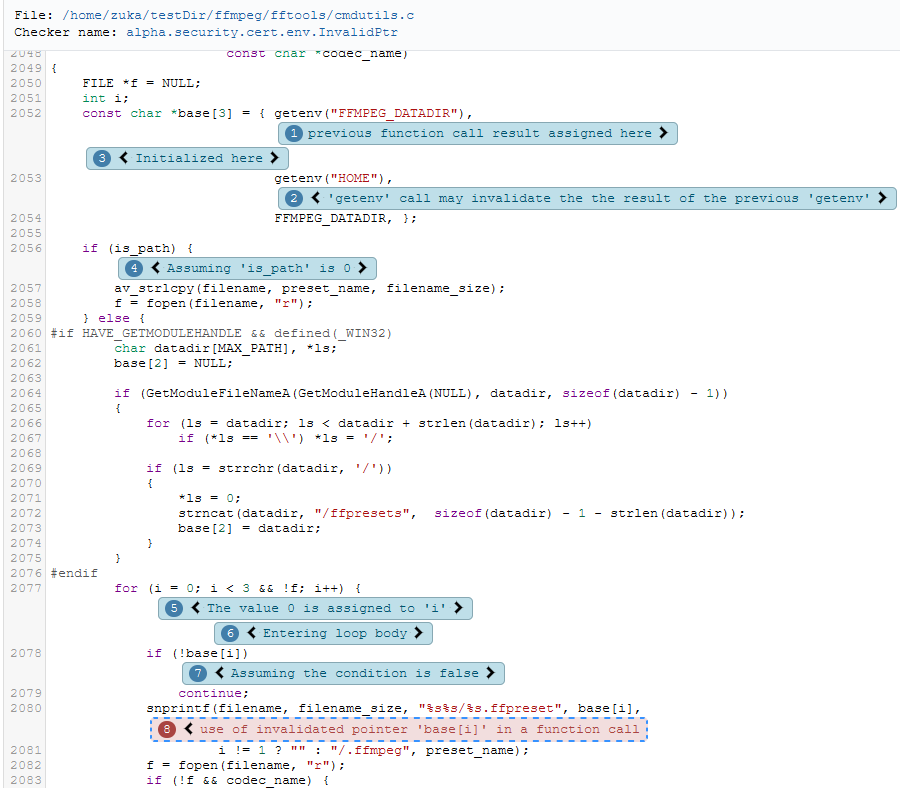
\includegraphics[width=\textwidth]{images/ffmpeg.png}
	\caption{Invalidated pointer usage in FFmpeg}
	\label{fig:ffmpeg-rep}
\end{figure}

\begin{figure}[H]
	\centering
	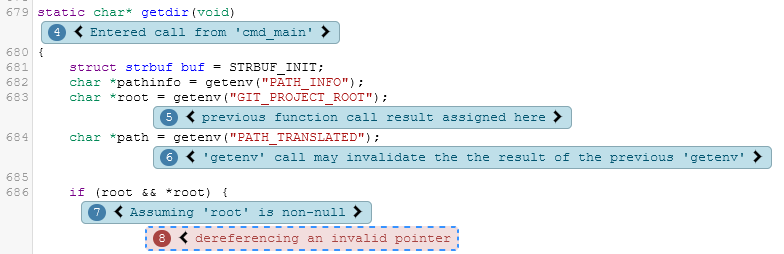
\includegraphics[width=\textwidth]{images/git_report.PNG}
	\caption{Invalidated pointer dereference in Git}
	\label{fig:git-rep}
\end{figure}

\cleardoublepage

\chapter{Conclusion and future work} % Conclusion
\label{ch:sum}


This thesis presented a solution to automate the detection of three different types of bugs in C and C++ codebases.
We developed two checkers for Clang Static Analyzer, an open-source static analysis tool.
The project was a success, and it met all of the original specifications.
One of the checkers has already passed the LLVM code review, demonstrating its high quality, and runs on millions of devices across the world as part of the Clang. Thesis documentation can be used as a guide by anyone who wishes to develop Clang Static Analyzer checkers. 

% In this thesis, we presented a solution to automate the detection of three different types of bugs in C and C++ codebases. We have created two checkers for the open-source static analysis tool - Clang Static Analyzer. The project was successful and meets the demands of all of the original specifications. One of the checkers already passed LLVM's code review, proving it's highest quality, and runs on millions of devices across the world as part of the Clang. 

Both checkers can be improved.
The InvalidPtr checker's short-term goal would be to successfully complete the LLVM review, later investigation should follow to extend it with more non-reentrant functions that suffer from similar problem, whereas the POS34 checker's goal would be to remove it from the so-called "alpha" state, i.e. enable it by default for all Clang Static Analyzer runs.
This could be accomplished by reducing the number of false positives, for example, by warning on the last \lstinline{putenv()} call on the execution path through the current stack frame.


% Both checkers can be further improved. Short term goal of the InvalidPtr checker would be to successfully conclude the review, while for POS34 checker aim is to take it out from the so-called "alpha" state, i.e. enable it by default for all Clang Static Analyzer runs. This could be achieved by reducing the number of false positives, for example, by warning on the last \lstinline{putenv} call on the execution path through the current stack frame.

Overall, this project is not only my favorite topic in program analysis, but it is also an excellent choice for demonstrating knowledge gained throughout my bachelor's degree studies.


\section*{Acknowledgements}
I would like to thank the following people, without whom I would not have been able to complete this thesis, and without whom I would not have made it through my bachelor degree! 

First and foremost, I'd like to thank my supervisor, Prof. Zoltán Porkoláb, for assisting me in selecting a thesis topic and guiding me through the process of writing thesis work. 

I would also like to extend my deepest gratitude to to Balázs Benics (ELTE, Ericsson) and Csaba Dabis (ELTE) for assisting with the design of the checkers, as well as answering all of my questions during the development phase, dedicating time for one-on-one meetings even on weekends, debugging the code with me, and suggesting how to further polish the work for the LLVM submission. 

Special thanks to Ericsson's CodeChecker team for their valuable suggestions during the early phase of the checkers. And to my team at Ericsson -- CI Joe, for giving me the flexibility and time needed to work on this thesis. 

Many thanks to Prof. Zoltán Gera for mentoring and introducing me to the Clang in Security Checker Development lab, as well as for teaching Imperative Programming during the first semester of my bachelor studies, the subject that served as the foundation for my C++ and C knowledge. 

I would also like to acknowledge Prof. Viktoria Zsók, who first introduced me to doing research early at my bachelor studies. Writing a thesis was made much easier because of previous experience. 

I am also grateful to LLVM reviewers: Artem Dergachev (Apple Inc.), Kristóf Umann (ELTE, Ericsson), and Aaron Ballman (Intel Corp.), for their insightful comments on the code and for making it possible that part of my thesis runs on millions of devices worldwide as part of Clang.

\cleardoublepage

% Függelékek (opcionális) - hosszabb részletező táblázatok, sok és/vagy nagy kép esetén hasznos
% Appendices (optional) - useful for detailed information in long tables, many and/or large figures, etc.
\appendix
\chapter{Szimulációs eredmények} % Simulation results
\label{appx:simulation}

Lorem ipsum dolor sit amet, consectetur adipiscing elit. Pellentesque facilisis in nibh auctor molestie. Donec porta tortor mauris. Cras in lacus in purus ultricies blandit. Proin dolor erat, pulvinar posuere orci ac, eleifend ultrices libero. Donec elementum et elit a ullamcorper. Nunc tincidunt, lorem et consectetur tincidunt, ante sapien scelerisque neque, eu bibendum felis augue non est. Maecenas nibh arcu, ultrices et libero id, egestas tempus mauris. Etiam iaculis dui nec augue venenatis, fermentum posuere justo congue. Nullam sit amet porttitor sem, at porttitor augue. Proin bibendum justo at ornare efficitur. Donec tempor turpis ligula, vitae viverra felis finibus eu. Curabitur sed libero ac urna condimentum gravida. Donec tincidunt neque sit amet neque luctus auctor vel eget tortor. Integer dignissim, urna ut lobortis volutpat, justo nunc convallis diam, sit amet vulputate erat eros eu velit. Mauris porttitor dictum ante, commodo facilisis ex suscipit sed.

Sed egestas dapibus nisl, vitae fringilla justo. Donec eget condimentum lectus, molestie mattis nunc. Nulla ac faucibus dui. Nullam a congue erat. Ut accumsan sed sapien quis porttitor. Ut pellentesque, est ac posuere pulvinar, tortor mauris fermentum nulla, sit amet fringilla sapien sapien quis velit. Integer accumsan placerat lorem, eu aliquam urna consectetur eget. In ligula orci, dignissim sed consequat ac, porta at metus. Phasellus ipsum tellus, molestie ut lacus tempus, rutrum convallis elit. Suspendisse arcu orci, luctus vitae ultricies quis, bibendum sed elit. Vivamus at sem maximus leo placerat gravida semper vel mi. Etiam hendrerit sed massa ut lacinia. Morbi varius libero odio, sit amet auctor nunc interdum sit amet.

Aenean non mauris accumsan, rutrum nisi non, porttitor enim. Maecenas vel tortor ex. Proin vulputate tellus luctus egestas fermentum. In nec lobortis risus, sit amet tincidunt purus. Nam id turpis venenatis, vehicula nisl sed, ultricies nibh. Suspendisse in libero nec nisi tempor vestibulum. Integer eu dui congue enim venenatis lobortis. Donec sed elementum nunc. Nulla facilisi. Maecenas cursus id lorem et finibus. Sed fermentum molestie erat, nec tempor lorem facilisis cursus. In vel nulla id orci fringilla facilisis. Cras non bibendum odio, ac vestibulum ex. Donec turpis urna, tincidunt ut mi eu, finibus facilisis lorem. Praesent posuere nisl nec dui accumsan, sed interdum odio malesuada.
\cleardoublepage

% Irodalomjegyzék (kötelező)
% Bibliography (mandatory)
\addcontentsline{toc}{chapter}{\biblabel}
\printbibliography[title=\biblabel]
\cleardoublepage

% Ábrajegyzék (opcionális) - 3-5 ábra fölött érdemes
% List of figures (optional) - useful over 3-5 figures
\addcontentsline{toc}{chapter}{\lstfigurelabel}
\listoffigures
\cleardoublepage

% Táblázatjegyzék (opcionális) - 3-5 táblázat fölött érdemes
% List of tables (optional) - useful over 3-5 tables
\addcontentsline{toc}{chapter}{\lsttablelabel}
\listoftables
\cleardoublepage

% Forráskódjegyzék (opcionális) - 3-5 kódpélda fölött érdemes
% List of codes (optional) - useful over 3-5 code samples
\addcontentsline{toc}{chapter}{\lstcodelabel}
\lstlistoflistings
\cleardoublepage

% Jelölésjegyzék (opcionális)
% List of symbols (optional)
%\printnomenclature

\end{document}
